\section{Initial situation and problem definition}

The company Siemens develops a system called Siemens GNA for many customers both within and outside of Austria, which constantly monitors and guarantees the reliability of the power grid. Due to the numerous elements such as busbars, surge arresters, generators, transformers, disconnectors, circuit breakers, stations, fuses, and load break switches, this utility grid consists of highly complex data. Additionally, with so many elements, it is easy for certain errors, usually in the form of deviations from set values, to occur in the network model. These errors are detected by Siemens, but currently, there is no application available to efficiently process and visualize these collected error data.

Engineers at Siemens analyze the errors using simple text files, which are difficult to read and unnecessarily prolong the duration of repair in the event of a major outage. To make the analysis of error data more efficient, Clemens Schlipfinger and Felix Schneider are developing an application that visualizes these interconnected data with optimal visualization methods. In this work, they focus particularly on the design of a decoupled backend system, which is implemented in the prototype using Apache Kafka, and some suitable visualization methods for such complex data.

As you can see, the illustration \ref{fig:architecture_introduction} visualizes the architecture of our system. First, the fault data is generated by a piece of software from Siemens, which is called GNA (\emph{Global Network Analysis}) and transported to the backend over a fail-safe Apache Kafka system. This message bus decouples our system and the software from Siemens even more and enhances the reliability. Subsequently, the data is saved into a relational database called PostgreSQL. The GraphQL API provides an interface for the frontend application, which is based on the JavaScript-Framework Angular. The frontend offers great visualizations and filters in order to provide intuitive information.

\begin{figure}
    \centering
    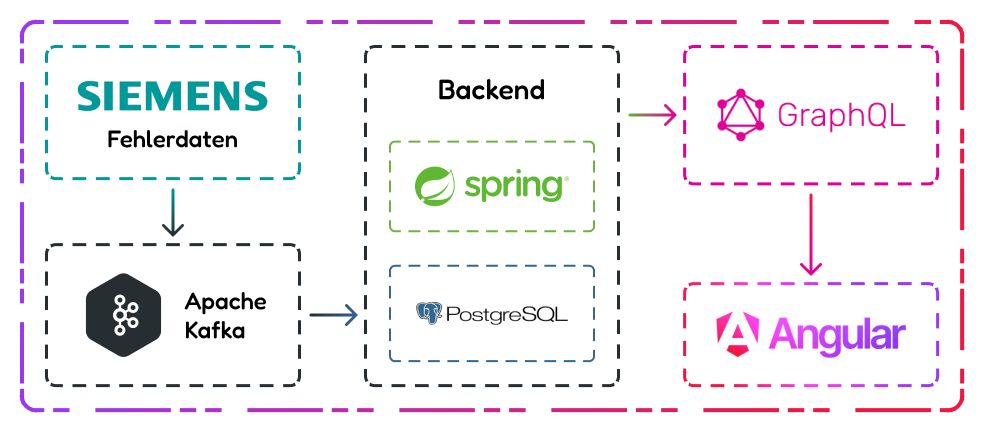
\includegraphics[width=0.8\textwidth]{content/img/Architecture/Architecture.jpg}
    \caption{This illustration shows the architecture of our application.}
    \label{fig:architecture_introduction}
\end{figure}
\FloatBarrier